To find such an example of an area where the focus on performance never really waned, let us examine the evolution of the computing that goes into making computing itself possible, which is the electronic design automation (EDA) tools that are used to design computers themselves.

If we took the computations that went into designing, simulating, or verifying a particular microchip in 2010 and ran the same workload every year since, we would see something like this:

\hspace*{\fill} \\ %插入空行
\begin{center}
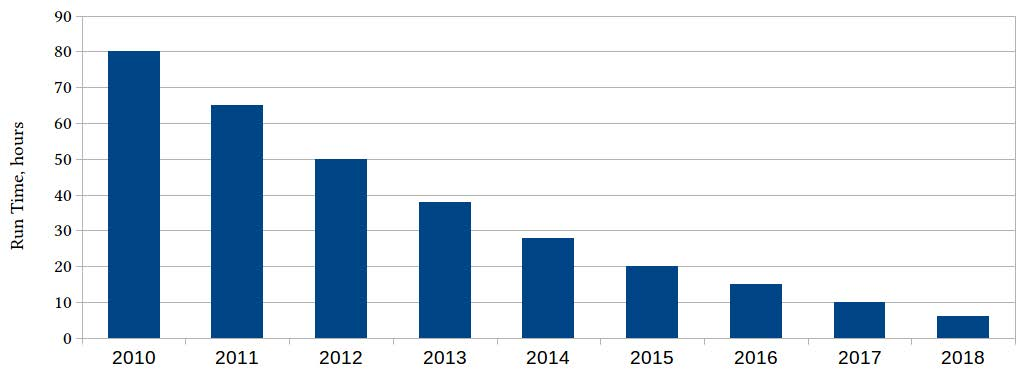
\includegraphics[width=0.9\textwidth]{content/1/chapter1/images/2.jpg}\\
Figure 1.2 – Processing time, in hours, for a particular EDA computation, over the years
\end{center}

What took 80 hours to compute in 2010 took less than 10 hours in 2018 (and even less today). Where does the improvement come from? Several sources at once: in part, computers become faster, but also software becomes more efficient, better algorithms are invented, the optimizing compilers become more effective.

Unfortunately, we are not building 2010 version microchips in 2021: it stands to reason that as computers become more powerful, building newer and better ones becomes harder. The more interesting question, then, is how long does it take to do the same work every year for the new microchip we're building that year:

\hspace*{\fill} \\ %插入空行
\begin{center}
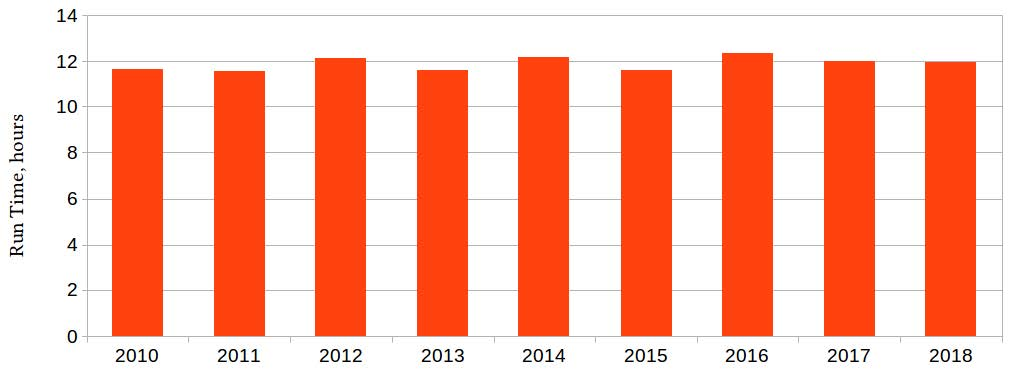
\includegraphics[width=0.9\textwidth]{content/1/chapter1/images/3.jpg}\\
Figure 1.3 – Run time, in hours, for a particular design step for the latest microchip every year
\end{center}

The actual computations done each year are not the same, but they serve the same purpose, for example, verify that the chip performs as intended, for the latest and greatest chip we built every year. We can see from this chart that the most powerful processors of the current generation, running the best tools available, take roughly the same time to design and model the processor of the next generation every year. We are holding our own, but we are not making any headway.

But the truth is even worse than that, and the chart above does not show everything. It is true that from 2010 to 2018, the largest processor to be made that year could be verified overnight (some 12 hours) using the computer equipped with the largest processors made last year. But we forgot to ask how many of these processors? Well, here is the full truth now:

\hspace*{\fill} \\ %插入空行
\begin{center}
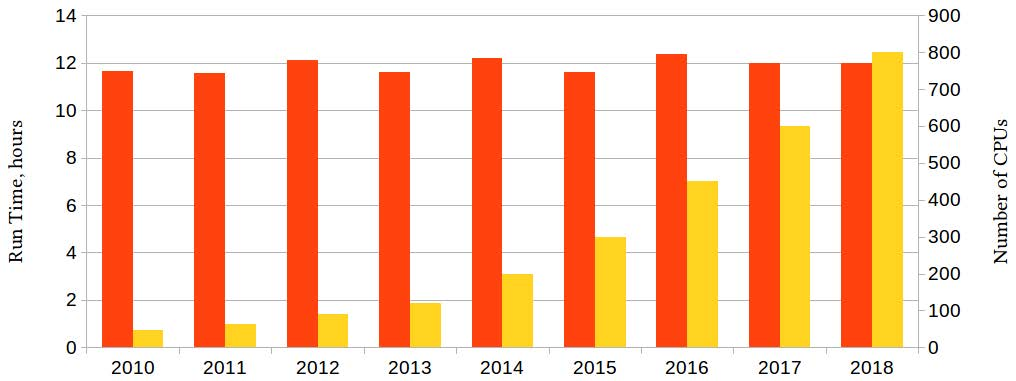
\includegraphics[width=0.9\textwidth]{content/1/chapter1/images/4.jpg}\\
Figure 1.4 – The preceding figure, annotated with the CPU count for each computation
\end{center}

Every year, the most powerful computers, equipped with the ever-growing number of the latest, most powerful processors, running the latest software versions (optimized to leverage increasingly more processors and to use each one more efficiently), do the work needed to build the next year's most powerful computers, and every year, this task is balanced on the edge of what is barely possible. That we do not fall off this edge is largely the achievement of the hardware and the software engineers, as the former supply the growing compute power, and the latter use it with maximum efficiency. This book will help you to learn the skills for the latter.

We now understand the importance of the subject of the book. Before we can delve into the details, it would help to do a high-level overview; a review of the map of the territory where the exploration campaign will unfold, so to speak.


















